% !TEX root = B&G_oefeningen.tex
\chapter{Binaire bomen en zoekbomen - Verdieping}

%Hier komen een aantal oefeningen op BST, verzameld uit examenvragen van voorbije jaren.
%\\
%
%Ook mogelijk om decodering van morse-tekens als oefening te implementeren, zie morse.zip in week03-04 of https://www.mathworks.com/content/dam/mathworks/mathworks-dot-com/moler/exm/chapters/morse.pdf. In het java-project is er ook documentatie opgenomen.  
%\\
%
%Zie ook map 1819: daar zijn reeds enkele bestanden met herhalingsoefeningen

In dit hoofdstuk vind je verdiepingsoefeningen bij de les `Bomen' enerzijds en de les `Binaire zoekbomen' anderzijds. Er zijn zowel theorie- als praktijkoefeningen. De praktijkoefeningen zijn vaak extra methodes die je aan de domain-klassen van de vorige hoofdstukken kan toevoegen.


\begin{oef}\papier \emph{(Examenvraag augustus 2019)}
%oplossing: https://www.geeksforgeeks.org/data-structures-binary-trees-question-1/
Je weet wat een complete binaire boom is. Een \emph{strikt} binaire boom wordt gedefinieerd als een binaire boom waar elke knoop, met uitzondering van de bladeren, \emph{exact twee} kinderen heeft. Je krijgt nu 5 stellingen over beide bomen. Welke van de 5 stellingen is juist? \emph{Geef bij elke stelling die je af- of goedkeurt een duidelijke uitleg mbv een figuur.}
\begin{enumerate}
\item Elke binaire boom is ofwel compleet ofwel strikt.
\item Elke complete binaire boom is ook een strikt binaire boom.
\item Elke strikt binaire boom is ook een complete binaire boom.
\item Een binaire boom kan nooit tegelijk compleet en strikt zijn.
\item Geen enkele van bovenstaande zinnen is juist.
\end{enumerate}
\begin{opl}
De laatste stelling is juist, nl. geen van de vier vorige is correct. Figuur~\ref{fig:tegenvoorbeelden} toont voor elke van deze vier stellingen een tegenvoorbeeld.
\begin{figure}[htbp]
    \centering
    \begin{subfigure}[b]{0.45\textwidth}
        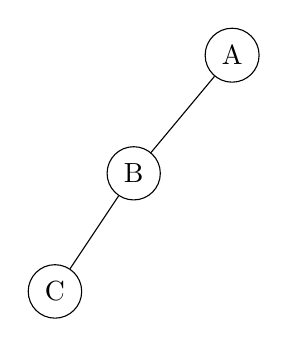
\begin{tikzpicture}[every node/.style={circle,draw},
				level 1/.style={sibling distance=25mm},
				level 2/.style={sibling distance=20mm}]
\node {A}
child { node {B} 
	child { node {C} }
	child[missing]
		 }
child[missing]
;
\end{tikzpicture}
        \caption{niet compleet, niet strikt}
        \label{fig:nietcompleetnietstrikt}
    \end{subfigure}
    ~ 
       \begin{subfigure}[b]{0.45\textwidth}
        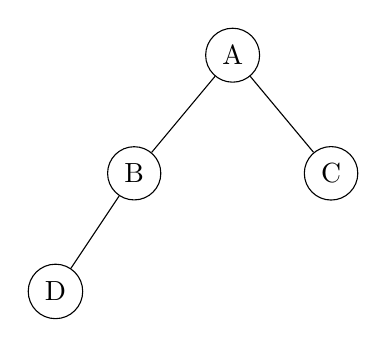
\begin{tikzpicture}[every node/.style={circle,draw},
				level 1/.style={sibling distance=25mm},
				level 2/.style={sibling distance=20mm}]
\node {A}
child { node {B} 
	child { node {D} }
	child[missing]
		 }
child { node {C} }
;
\end{tikzpicture}
        \caption{compleet maar niet strikt}
        \label{fig:compleetnietstrikt}
    \end{subfigure}
    
          \begin{subfigure}[b]{0.45\textwidth}
        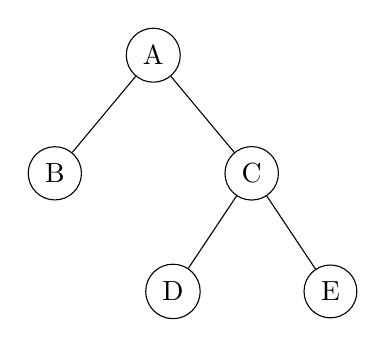
\begin{tikzpicture}[every node/.style={circle,draw},
				level 1/.style={sibling distance=25mm},
				level 2/.style={sibling distance=20mm}]
\node {A}
child { node {B} }
child { node {C}
	child { node {D} }
	child { node {E} }
	}
;
\end{tikzpicture}
        \caption{strikt maar niet compleet}
        \label{fig:striktnietcompleet}
    \end{subfigure}
    ~
    \begin{subfigure}[b]{0.45\textwidth}
        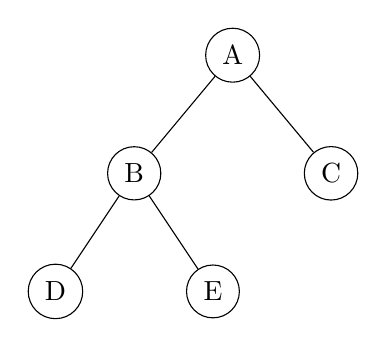
\begin{tikzpicture}[every node/.style={circle,draw},
				level 1/.style={sibling distance=25mm},
				level 2/.style={sibling distance=20mm}]
\node {A}
child { node {B} 
	child { node {D} }
	child { node {E} }
	}
child { node {C} }
;
\end{tikzpicture}
        \caption{strikt en compleet}
        \label{fig:striktcompleet}
    \end{subfigure}
    \caption{Tegenvoorbeelden voor de stellingen 1 t.e.m. 4}
    \label{fig:tegenvoorbeelden}
\end{figure}
\end{opl}
\end{oef}



\begin{oef}
\code Gegeven de implementatie van een binaire boom zoals in les 2 gegeven.
De bedoeling van deze oefening is het aantal voorkomens van een gegeven data-veld in een binaire boom te tellen.
\begin{oefenumerate}
\item Implementeer een methode \verb+count+ in de \verb+BinaryTree+ klasse die het aantal voorkomens van een gegeven data-veld telt in een boom.
\item Maak een nieuwe \verb+BinaryTreeDriver+ klasse waarin je de boom overeenkomstig figuur~\ref{fig:herhalingsoefbb} maakt.
\begin{figure}[htbp]
    \centering
\begin{tikzpicture}[every node/.style={circle,draw},
				level 1/.style={sibling distance=50mm},
				level 2/.style={sibling distance=30mm},
				level 3/.style={sibling distance=20mm},
				level 4/.style={sibling distance=10mm}]
\node {A}
child { node {H} 
	child { node {A} }
	child { node {H} 
		child { node {C}
			child[missing]
			child { node {E}}
		 } 
		child { node {E} } }
}
child { node {G}
	child[missing]
	child { node {I}
		child { node {H}
			child[missing]
			child { node {E}}
		}
		child { node {E}}
		}
	};
\end{tikzpicture}

\caption{Binaire boom met herhaalde datavelden}
    \label{fig:herhalingsoefbb}
\end{figure}
\item Run de main functie in de \verb+BinaryTreeDriver+ klasse en controleer hiermee de implementatie van de \verb+count+ methode met respectievelijke parameters: I, A, H, E en Q.
Verwachte uitvoer:\\
Aantal voorkomen van I = 1\\
Aantal voorkomens van A = 2\\
Aantal voorkomens van H = 3\\
Aantal voorkomens van E = 4\\
Aantal voorkomens van Q = 0\\
\end{oefenumerate}
\begin{opl}
\begin{lstlisting}[caption={count methode}, label=herhoefbbcount]
public int count(E geg) {
	if (geg == null) {
		return 0;
	}
	return (this.data.equals(geg) ? 1 : 0) 
			+ (this.leftTree != null ? this.leftTree.count(geg) : 0) 
			+ (this.rightTree != null ? this.rightTree.count(geg) : 0);
}
\end{lstlisting}
\end{opl}
\end{oef}


\begin{oef}
\papier \emph{(Examen augustus 2019)} Een preorder wandeling in een binaire zoekboom (BST) met in de knopen gehele getallen levert als resultaat volgende rij: 30, 20, 10, 15, 25, 23, 39, 35, 42. Geef het resultaat van een postorder wandeling in dezelfde BST.

\begin{opl}
% oplossing: https://www.geeksforgeeks.org/data-structures-binary-search-trees-question-8/
Postorder geeft: 15, 10, 23, 25, 20, 35, 42, 39, 30

Gebruik de preorder wandeling om de gevraagde boom te tekenen.
\end{opl}
\end{oef}


\begin{oef}
\papier \emph{(Examen augustus 2019)} Men zoekt in een BST van gehele getallen naar het getal 43. Men doorloopt zo een aantal knopen en het zesde getal is 43. Welke van volgende rijen van getallen zijn \emph{niet} mogelijk als lijst van opeenvolgende knopen die men bekomt als resultaat van de zoektocht? Geef een duidelijke uitleg waarom je antwoord(en) niet kan (kunnen).
\begin{enumerate}
\item 61, 52, 14, 17, 40, 43
\item 2, 3, 50, 40, 60, 43
\item 10, 65, 31, 48, 37, 43
\item 81, 61, 52, 14, 41, 43
\item 17, 77, 27, 66, 18, 43
\end{enumerate}
\begin{opl}
% oplossing: https://www.geeksforgeeks.org/gate-gate-cs-1996-question-52/
Mogelijke oplossingen: nr 1, 3 en 4
\begin{itemize}
\item In nr 2 kan je knoop 60 niet tegenkomen in de zoektocht naar 43 want knoop 60 moet rechts van knoop 50 komen terwijl knoop 43 links moet staan.
\item In nr 5 kan je knoop 18 niet tegenkomen omdat deze knoop links moet staan van knoop 27 terwijl je knoop 43 rechts moet zoeken.
\end{itemize}
\end{opl}
\end{oef}




\begin{oef}
\code Zoek de knopen op een bepaalde afstand.
\begin{oefenumerate}
\item Schrijf een methode \verb=getNodesAtDistance(k)= in de \verb+BinaryTree+ klasse die een lijst teruggeeft van de datavelden die op een afstand $k$ van de wortel van de binaire boom verwijderd zijn. In de boom uit figuur~\ref{fig:herhalingsoefbb} zijn A, H en I de datavelden van knopen die op een afstand 2 van de root verwijderd zijn.
\item Test je implementatie uit door in de klasse \verb+BBDriver+ de methode \verb+getNodesAtDistance+ op te roepen met parameters 0, 1, 2, 3 en 4. Verwachte uitvoer: \\
Datavelden van knopen verwijderd op een afstand van 0 van de root = [A]\\
Datavelden van knopen verwijderd op een afstand van 1 van de root = [H, G]\\
Datavelden van knopen verwijderd op een afstand van 2 van de root = [A, H, I]\\
Datavelden van knopen verwijderd op een afstand van 3 van de root = [C, E, H, E]\\
Datavelden van knopen verwijderd op een afstand van 4 van de root = [E, E]
\end{oefenumerate}

\begin{opl}
\begin{lstlisting}[caption={getNodesAtDistance(k) methode}, label=herhoefbbdistance]
public ArrayList<E> getNodesAtDistance(int k) {
	if (k < 0) {
		throw new IllegalArgumentException("Foute waarde voor afstand!");
	}
	ArrayList<E> res = new ArrayList<>();
	if (k == 0) {
		res.add(this.data);
	} else {
		if (this.leftTree != null) {
			res = this.leftTree.getNodesAtDistance(k - 1);
		}
		if (this.rightTree != null) {
			ArrayList<E> rechtsteLijst = this.rightTree.getNodesAtDistance(k - 1);
			res.addAll(rechtsteLijst);
		}
	}
	return res;
}
\end{lstlisting}
\end{opl}
\end{oef}


\begin{oef}
\papier Gegeven volgende code:
\begin{lstlisting}[caption={Mystery methode}, label=herhoefmystery]
public ArrayList<E> mystery() {
	ArrayList<E> lijst = new ArrayList<>();
	if (this.leftTree != null) lijst.add(this.leftTree.data);
	if (this.rightTree != null) lijst.add(this.rightTree.data);
	return lijst;
}

public ArrayList<E> mystery(int g) {
	if (g == 1) {
		return this.mystery();
	} else {
		ArrayList<E> links = new ArrayList<>();
		if (this.leftTree != null) links = this.leftTree.mystery(g - 1);
		ArrayList<E> rechts = new ArrayList<>();
		if (this.rightTree != null) rechts = this.rightTree.mystery(g - 1);
		links.addAll(rechts);
		return links;
	}
}
 \end{lstlisting}
 Geef nu de uitvoer van volgende oproepen van deze methode voor de boom uit figuur~\ref{fig:herhalingsoefbb}:
 \begin{oefenumerate}
 \item \verb+boom.mystery(1)+
 \item \verb+boom.mystery(2)+
 \item \verb+boom.mystery(3)+
 \item \verb+boom.mystery(4)+
 \item \verb+boom.mystery(5)+
 \end{oefenumerate}

\begin{opl}
Je had al door dat dit een andere manier is om de vorige oefening in een opgave te gieten, niet?
\end{opl}
\end{oef}




\begin{oef}
\code \emph{(Examen juni 2017)} Schrijf een methode \verb+kinderSom()+. Het resultaat is een boolean. De methode geeft true terug als de boom waarop ze toegepast wordt voldoet aan de eigenschap dat elke knoop als waarde de som van zijn kinderen heeft (dat aantal kinderen kan natuurlijk 2, 1 of 0 zijn). Figuur~\ref{fig:herhalingsoefbbkindersom} op pagina~\pageref{fig:herhalingsoefbbkindersom} toont een boom die aan deze eigenschap voldoet.

Je zal voor deze methode een nieuwe klasse moeten schrijven. Je kan immers niet zomaar de waarde van twee knopen van een nog te bepalen type \verb+E+ optellen, bvb. als je voor \verb+E+ het type \verb+String+ kiest! Beperk je dus voor deze oefening tot een nieuw soort binaire boom, nl. één waarbij het veld \verb+data+ een \verb+int+ is. Test je methode uit door de boom van figuur~\ref{fig:herhalingsoefbbkindersom} te implementeren in een mainmethode en het resultaat van de toepassing van deze methode op deze boom naar de console te schrijven.
\begin{figure}[htbp]
    \centering
\begin{tikzpicture}[every node/.style={draw},
				level 1/.style={sibling distance=50mm},
				level 2/.style={sibling distance=30mm},
				level 3/.style={sibling distance=15mm}]
\node {7}
child { node {4} 
	child { node {5}
		child {node {8}}
		child { node {$-3$}}
	 }
	child { node {$-1$} 
		child { node {$-1$}} 
		child[missing]  
	}
}
child { node {3}
	child { node {0}}
	child { node {3}
		child { node {10}}
		child { node {$-7$}}
		}
};
\end{tikzpicture}
\caption{Binaire boom voldoet aan kinderSom}
    \label{fig:herhalingsoefbbkindersom}
\end{figure}
\begin{opl}
	\begin{lstlisting}[caption={kinderSom() methode}, label=kinderSom]
	
public class BinaryTreeInt {

private int data;
private BinaryTreeInt leftTree, rightTree;

public BinaryTreeInt(int data) {
	this(data, null, null);
}

public BinaryTreeInt(int data, BinaryTreeInt leftTree, BinaryTreeInt rightTree) {
	this.data = data;
	this.leftTree = leftTree;
	this.rightTree = rightTree;
}
	
public boolean kinderSom() {
	// Controleer of wortel voldoet aan voorwaarden van kindersom
	// Als wortel een blaadje is, voldoet hij 
	if (this.isLeaf())
		// bij een blaadje is kinderSom altijd true
		return true;
	// Als wortel geen blaadje is: controle uitvoeren
	else {
		// Bereken som van de waardes van de kinderen
		// De somwaarde van een kind is gelijk aan zijn waarde, 
		// tenzij het kind niet bestaat. Dan is de somwaarde gelijk aan 0
		int left_value = (this.leftTree != null ? this.leftTree.data : 0);
		int right_value = (this.rightTree != null ? this.rightTree.data : 0);
		// Als de som niet juist is, voldoet de boom niet aan de voorwaarden
		// Methode kan afgebroken worden
		if (this.data != left_value + right_value)
			return false;
	}
	
	// Als wortel wel voldoet aan voorwaarden, moet de rest van de boom gecontroleerd worden
	return (this.leftTree != null ? this.leftTree.kinderSom() : true) && 
		(this.rightTree != null ? this.rightTree.kinderSom() : true);
}

...
}
	\end{lstlisting}
\end{opl}
	
\end{oef}


\begin{oef}
\papier \emph{(Examen juni 2019)}Een binaire boom heeft een letter als waarde in elke knoop. Als je de boom \emph{in-order} doorwandelt krijg je ‘FHCADEGB’. Een \emph{post-order} wandeling levert voor dezelfde boom ‘FCHAGEBD’. Teken hieronder deze boom.
\begin{opl}

Deze boom kun je bekomen door volgend stappenplan:
\begin{enumerate}
	\item In \emph{post-order} staat de root van de boom altijd achteraan.
	\item Kijk in de \emph{in-order} wandeling waar dat de root zich bevindt. Alles links van de root is de linker sub-boom en alles recht van de root is de rechter sub-boom.
	\item Herhaal deze stappen opnieuw voor de linker en de rechter sub-boom.
\end{enumerate}

Concreet voor deze opgave betekend dit:
\begin{enumerate}
	\item Voor de gehele boom in \emph{post-order} zien we dat ‘D’ achteraan staat en dus de root van onze boom gaat zijn.
	\item De linker subboom bestaat uit ‘FHCA’ \emph{in-order} en de rechter subboom uit ‘EGB’ \emph{in-order}.
	\item De linker subboom in \emph{post-order} bestaat uit ‘FCHA’ en de rechter subboom in \emph{post-order} bestaan uit ‘GEB’.
	\item Voor de linker subboom in \emph{post-order} zien we dat ‘A’ achteraan staat en dus de root van onze subboom gaat zijn.
	\item De linker sub-subboom bestaat uit ‘FHC’ \emph{in-order} en de rechter sub-subboom is leeg.
	\item De linker sub-subboom in \emph{post-order} bestaat uit ‘FCH’ en de rechter sub-subboom is nog steeds leeg.
	\item Voor de linker sub-subboom in \emph{post-order} zien we dat ‘H’ achteraan staat en dus de root van onze volgende subboom gaat zijn.
	\item Blijft dit herhalen tot links en rechts geen subbomen meer hebben.
\end{enumerate}
Figuur~\ref{fig:exjuni19inpost} op pagina~\pageref{fig:exjuni19inpost} toont de boom.
\begin{figure}[htbp]
    \centering
\begin{tikzpicture}[every node/.style={circle,draw},
				level 1/.style={sibling distance=50mm},
				level 2/.style={sibling distance=30mm},
				level 3/.style={sibling distance=20mm}]
\node {D}
child { node {A} 
	child { node {H}
		child { node {F} }
		child {node {C} } 
	}
	child[missing]
}
child { node {B}
	child { node {E}
		child[missing]
		child { node {G} }	
	}
	child[missing]
};
\end{tikzpicture}
\caption{Binaire boom horend bij de gegeven in en post-order uitvoer}
    \label{fig:exjuni19inpost}
\end{figure}
\end{opl}
\end{oef}


\begin{oef}
\papier De \verb+preorder+ methode van een BST geeft volgende uitvoer: 30, 20, 10, 15, 25, 23, 39, 35, 42.
Geef de \verb+postorder+ uitvoer.
\begin{opl}
Steun op de eigenschappen van een BST: een binaire boom, met alle knopen links van een knooppunt kleiner dan dit knooppunt en in de rechterboom van het knooppunt allemaal waarden die groter zijn. Je bekomt dan de boom in figuur~\ref{fig:herhoefBST1}. Kijk na dat die inderdaad de gegeven pre-order volgorde geeft. Als je nu op deze BST de post-order wandeling doet bekom als uitvoer: 15, 10, 23, 25, 20, 35, 42, 39, 30.
\begin{figure}[htbp]
    \centering
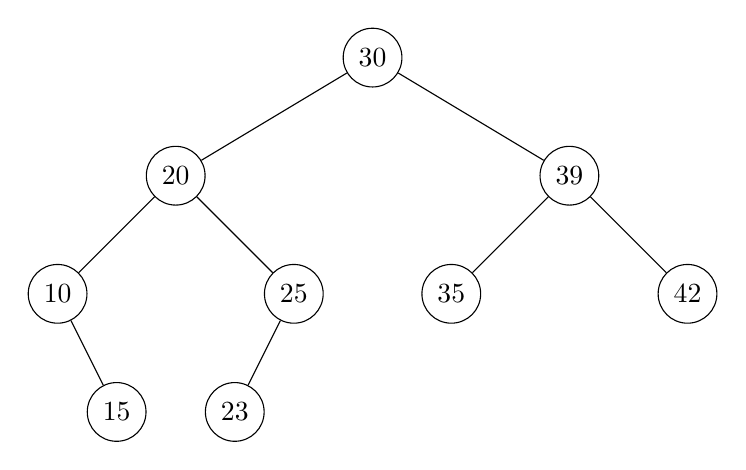
\begin{tikzpicture}[every node/.style={circle,draw},
				level 1/.style={sibling distance=50mm},
				level 2/.style={sibling distance=30mm},
				level 3/.style={sibling distance=15mm}]
\node {30}
child { node {20} 
	child { node {10}
		child[missing]
		child {node {15}}
		 }
	child { node {25} 
		child { node {23} } 
		child[missing]}
}
child { node {39}
	child { node {35}}
	child { node {42}}
};
\end{tikzpicture}
\caption{BST horend bij de gegeven pre-order uitvoer}
    \label{fig:herhoefBST1}
\end{figure}
\end{opl}

\end{oef}




\begin{oef}
\papier We wensen een BST te bouwen bestaande uit de gehele getallen 1 tot en met 10. In welke volgorde moeten de getallen worden toegevoegd opdat de resulterende boom compleet is?
\begin{opl}
Een goede manier om aan deze oefening te beginnen is een complete binaire boom tekenen met 10 knooppunten (figuur~\ref{fig:herhoefBST2Stap1}).
\begin{figure}[htbp]
    \centering
\begin{tikzpicture}[every node/.style={circle,draw},
				level 1/.style={sibling distance=50mm},
				level 2/.style={sibling distance=25mm},
				level 3/.style={sibling distance=13mm}]
\node {\phantom{7}}
child { node {\phantom{4}} 
	child { node {\phantom{2}}
		child { node {\phantom{1}}}
		child {node {\phantom{3}}}
		 }
	child { node {\phantom{6}} 
		child { node {\phantom{5}} } 
		child[missing]}
}
child { node {\phantom{9}}
	child { node {\phantom{8}}}
	child { node {\phantom{9}}}
};
\end{tikzpicture}
\caption{complete BST voor 10 getallen}
    \label{fig:herhoefBST2Stap1}
\end{figure}
Logisch redeneren met behulp van de basiskenmerken van een BST op deze blanco figuur levert in een aantal stappen de gewenste oplossing. Je kan bvb. volgende info gemakkelijk bekomen:
\begin{itemize}
\item links onderaan moet 1 staan (kleinste getal)
\item rechts onderaan moet 10 staan (grootste getal)
\item er zijn drie getallen groter dan de wortel, dus moet de wortel een 7 zijn
\item …
\end{itemize}
Je bekomt uiteindelijk figuur~\ref{fig:herhoefBST2Stap2}.
\begin{figure}[htbp]
    \centering
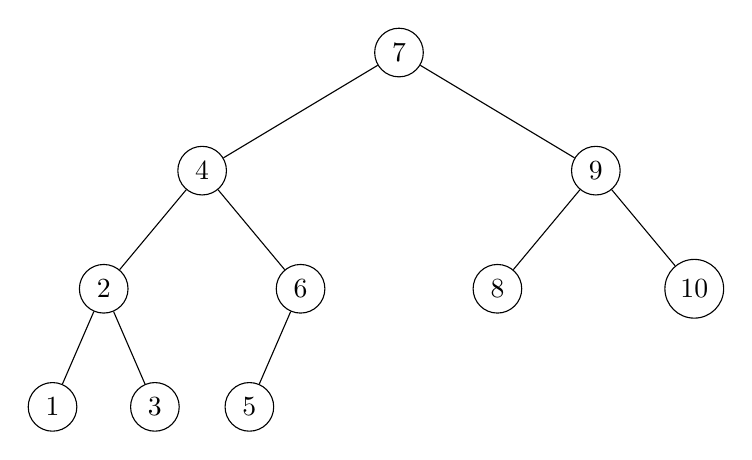
\begin{tikzpicture}[every node/.style={circle,draw},
				level 1/.style={sibling distance=50mm},
				level 2/.style={sibling distance=25mm},
				level 3/.style={sibling distance=13mm}]
\node {7}
child { node {4} 
	child { node {2}
		child { node {1}}
		child {node {3}}
		 }
	child { node {6} 
		child { node {5} } 
		child[missing]}
}
child { node {9}
	child { node {8}}
	child { node {10}}
};
\end{tikzpicture}
\caption{complete BST met getallen van 1 tot 10 ingevuld}
    \label{fig:herhoefBST2Stap2}
\end{figure}
Als je nu “laag per laag” aanvult komt alles waar het hoort te staan. De volgorde wordt dus: 7, 4, 9, 2, 6, 8, 10, 1, 3, 5, of liever gezegd “één van de mogelijke volgordes”. Snap je dat bvb. 7, 9, 4, … ook perfect mogelijk is?

\end{opl}

\end{oef}



\begin{oef}
\papier Stel dat 7, 5, 1, 8, 3, 6, 0, 9, 4 en 2 worden toegevoegd aan een lege BST. Wat is de diepte van de resulterende boom?
\begin{opl}
De resulterende boom heeft diepte 5 (figuur~\ref{fig:herhoefBST3}).
\begin{figure}[htbp]
    \centering
\begin{tikzpicture}[every node/.style={circle,draw},
				level 1/.style={sibling distance=45mm},
				level 2/.style={sibling distance=25mm},
				level 3/.style={sibling distance=18mm}]
\node {7}
child { node {5} 
	child { node {1}
		child { node {0}}
		child {node {3}
			child {node {2}}
			child {node {4}}
			}
		 }
	child { node {6}}
}
child { node {8}
	child[missing]
	child { node {9}}
};
\end{tikzpicture}
\caption{BST als resultaat van invullen in volgorde van 7, 5, 1, 8, 3, 6, 0, 9, 4 en 2}
    \label{fig:herhoefBST3}
\end{figure}
\end{opl}

\end{oef}



\begin{oef}
\papier Stel dat we een BST maken door vertrekkende van een lege BST vervolgens de getallen 71, 65, 84, 69, 67 en 83 toe te voegen. Welke zijn de data-velden van de bladeren van de boom?
\begin{opl}
De blaadjes van deze boom hebben als datavelden 67 en 83. De boom wordt getoond in figuur~\ref{fig:herhoefBST4}.
\begin{figure}[htbp]
    \centering
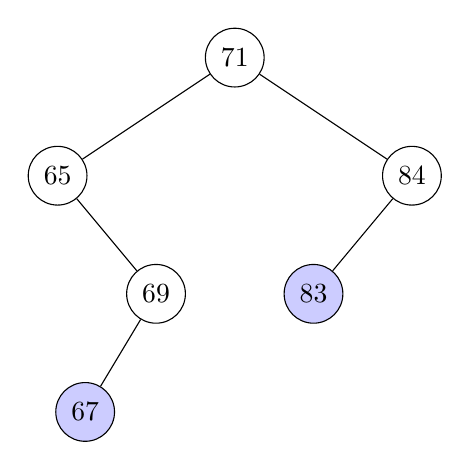
\begin{tikzpicture}[every node/.style={circle,draw},
				level 1/.style={sibling distance=45mm},
				level 2/.style={sibling distance=25mm},
				level 3/.style={sibling distance=18mm}]
\node {71}
child { node {65} 
	child[missing]
	child { node {69}
		child {node[fill=blue!20] {67}}
		child[missing]
	}
}
child { node {84}
	child { node[fill=blue!20]  {83}}
	child[missing]
};
\end{tikzpicture}
\caption{BST als resultaat van invullen in volgorde van 71, 65, 84, 69, 67 en 83}
    \label{fig:herhoefBST4}
\end{figure}
\end{opl}

\end{oef}



\begin{oef}
\papier Stel dat boom een BST is bestaande uit gehele getallen groter dan of gelijk aan 1 en kleiner dan of gelijk aan 100. Welke van de volgende paden kan (kunnen) niet?
\begin{oefenumerate}
\item 10, 75, 64, 43, 60, 57, 55
\item 90, 12, 68, 34, 62, 45, 55
\item 9, 85, 47, 68, 43, 57, 55
\item 79, 14, 72, 56, 16, 53, 55
\end{oefenumerate}
\begin{opl}
Pad 9, 85, 47, 68, 43, 57, 55 kan niet omdat $43 < 47$. Maak zelf de figuur, waarbij je telkens links of rechts gaat afhankelijk van of het nieuwe getal kleiner of groter is dan het vorige. Als je ergens naar rechts gaat, moeten alle getallen die daarna komen groter zijn dan dit vorige getal en die voorwaarde wordt hier geschonden.
\end{opl}
\end{oef}




\begin{oef}
\papier \emph{(Examenvraag juni 2017)}\\
\begin{enumerate}
\item Gegeven de binaire zoekboom (BST) in figuur~\ref{fig:bstex1}. 
\begin{itemize}
\item Vul een geheel getal in voor de ontbrekende knopen. 
\item Verbeter eventuele fouten (door enkel aanpassingen te doen aan de bladeren!), zodat de BST eigenschap voor deze boom volledig klopt.
\end{itemize}
\begin{figure}[htbp]
    \centering
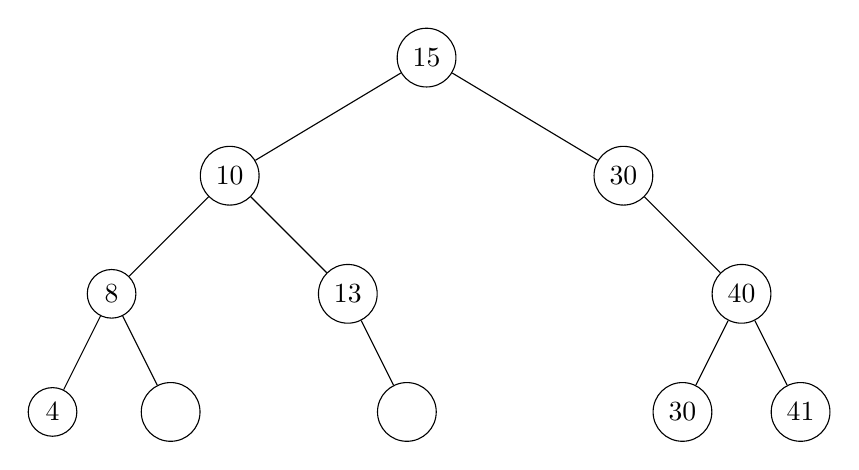
\begin{tikzpicture}[every node/.style={circle,draw},
				level 1/.style={sibling distance=50mm},
				level 2/.style={sibling distance=30mm},
				level 3/.style={sibling distance=15mm}]
\node {15}
child { node {10} 
	child { node {8} 
		child { node {4} } 
		child { node {\phantom{09}} }
		}
	child { node {13} 
		child[missing]  
		child { node {\phantom{14}} }
} }
child { node {30}
	child[missing]
	child { node {40}
		child { node {30} }
		child { node {41}}
	}
	};
\end{tikzpicture}
\vspace*{20mm}
\caption{}
    \label{fig:bstex1}
\end{figure}

\item Voeg aan de BST van figuur~\ref{fig:bstex1} een knoop met het getal 6 toe op de juiste plaats.
\item Vertrek nu van de boom die je in het vorige puntje bekwam. Teken hieronder de nieuwe toestand van de BST (teken de volledige boom) na verwijderen van de knoop met het getal 10.
\end{enumerate}

\begin{opl}
Figuur~\ref{fig:bstex1opl} op pagina~\pageref{fig:bstex1opl} toont de oplossing. In de plaats van het getal 35 mag elk geheel getal tussen 30 en 40 komen (grenzen 30 en 40 niet inbegrepen). Wat het verwijderen van de knoop met waarde 10 betreft: ofwel verdwijnt het blaadje met waarde 9 en komt de waarde in de knoop waar nu 10 staat. Ofwel schuift de knoop 13 eentje op en neemt de plaats in van de waarde 10.
\begin{figure}[htbp]
    \centering
\begin{tikzpicture}[every node/.style={circle,draw},
				level 1/.style={sibling distance=50mm},
				level 2/.style={sibling distance=35mm},
				level 3/.style={sibling distance=20mm},
				level 4/.style={sibling distance=10mm}]
\node {15}
child { node {10} 
	child { node {8} 
		child { node {4} 
			child[missing]
			child { node {6} }
		} 
		child { node {9} }
		}
	child { node {13} 
		child[missing]  
		child { node {14} }
} }
child { node {30}
	child[missing]
	child { node {40}
		child { node {35} }
		child { node {41}}
	}
	};
\end{tikzpicture}

\caption{Gewijzigde BST}
    \label{fig:bstex1opl}
\end{figure}
\end{opl}
\end{oef}







\begin{oef}
\papier \emph{(Examenvraag augustus 2017)}\\
\begin{enumerate}
\item Gegeven de binaire zoekboom (BST) in figuur~\ref{fig:bstex2}. Vul een letter in voor de ontbrekende knoop, zodat de BST eigenschap voor deze boom nog klopt.
\begin{figure}[htbp]
    \centering
\begin{tikzpicture}[every node/.style={circle,draw},
				level 1/.style={sibling distance=50mm},
				level 2/.style={sibling distance=30mm},
				level 3/.style={sibling distance=15mm}]
\node {K}
child { node {B} 
		child { node {A} } 
		child { node {D} }
		}
child{ node {M}
	child{ node {\phantom{14}} }
	child { node {Q}
		child { node {O} }
		child { node {S}}
	}
	};
\end{tikzpicture}
\caption{}
    \label{fig:bstex2}
\end{figure}
\item Voeg in figuur~\ref{fig:bstex2} aan de BST een knoop met dataveld C toe op de juiste plaats.
\item Teken de nieuwe toestand van de BST (teken de volledige boom, ook met dataveld C) na verwijderen van de knoop met het dataveld M.

\end{enumerate}

\begin{opl}
Figuur~\ref{fig:bstex2opl} op pagina~\pageref{fig:bstex2opl} toont de oplossing van de eerste twee vragen. Voor het antwoord op de derde vraag kan ofwel de knoop met waarde L ofwel de knoop met waarde O de plaats innemen van M.
\begin{figure}[htbp]
    \centering
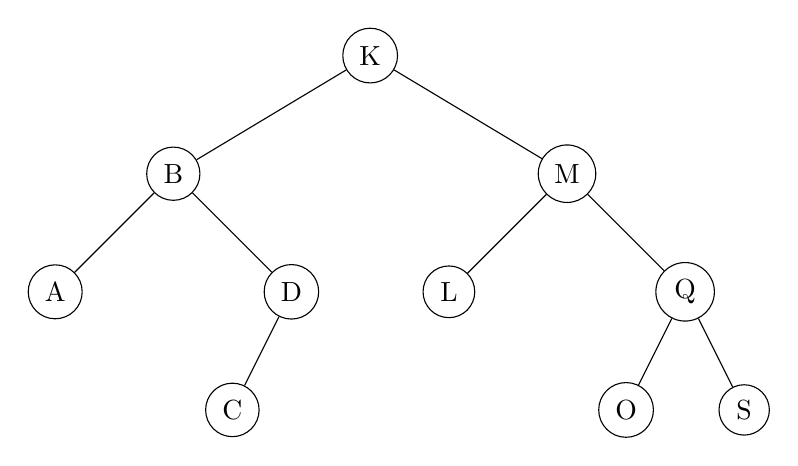
\begin{tikzpicture}[every node/.style={circle,draw},
				level 1/.style={sibling distance=50mm},
				level 2/.style={sibling distance=30mm},
				level 3/.style={sibling distance=15mm}]
\node {K}
child { node {B} 
		child { node {A} } 
		child { node {D} 
			child { node {C} }
			child[missing]
		}
}
child{ node {M}
	child{ node {L} }
	child { node {Q}
		child { node {O} }
		child { node {S}}
	}
};
\end{tikzpicture}
\caption{Gewijzigde BST}
    \label{fig:bstex2opl}
\end{figure}
\end{opl}
\end{oef}


\newpage
\begin{oef}
\papier \emph{(Examenvraag juni 2018)} Gegeven de volgende java-klasse:
\begin{lstlisting}
package domain;
public class Persoon implements Comparable<Persoon>{
	private String naam, voornaam;
	private int lengte;
	private double gewicht;
	public Persoon(String voornaam, String naam, int lengte, double gewicht) {
		this.setVoornaam(voornaam);
		this.setNaam(naam);
		this.setLengte(lengte);
		this.setGewicht(gewicht);
	}

	private void setNaam(String naam) {
		if (naam == null || naam.trim().isEmpty()) throw new
			 IllegalArgumentException();
		this.naam = naam;
	}

	private void setVoornaam(String voornaam) {
		if (voornaam == null || voornaam.trim().isEmpty()) throw new
			 IllegalArgumentException();
		this.voornaam = voornaam;
	}

	private void setLengte(int lengte) {
		if (lengte <= 30) throw new IllegalArgumentException();
		this.lengte = lengte;
	}

	private void setGewicht(double gewicht) {
		if (gewicht <= 25) throw new IllegalArgumentException();
		this.gewicht = gewicht;
	}
	
	public int getBMI() {
		return (int)(Math.round(gewicht * 10000 / (lengte * lengte)));
	}
	
	@Override
	public String toString() {
		return voornaam + " " + naam + " BMI = " + this.getBMI();
	}

	@Override
	public int compareTo(Persoon o) {
		if ( o == null) return 1;
		else {
			int i = this.getBMI() - o.getBMI();
			if (i != 0) return i;
			else {
				i = this.naam.compareTo(o.naam);
				if (i != 0) return i;
				else return this.voornaam.compareTo(o.voornaam);
			}
		}
	}
}
\end{lstlisting}
\begin{enumerate}
\item Volgende objecten worden aan een BST<Persoon> vervolgens toegevoegd:
\begin{verbatim}
els = new Persoon("Els","Adams",176,86) //bmi = 28	
an = new Persoon("Anne","Janssen",176,68) //bmi = 22
tom = new Persoon("Tom","Frederiks",185,105) // bmi = 31
tim = new Persoon("Tim","Anders",185,85) //bmi = 25
joke = new Persoon("Joke","Alders",176,86) //bmi = 28
\end{verbatim}
Teken de resulterende boomstructuur

\item  Hoeveel objecten zouden aan de boom uit het vorige puntje \emph{minimaal} moeten toegevoegd worden om deze \emph{compleet} te maken? Geef een concreet voorbeeld (zoals in bovenstaande code) voor elk van deze objecten.  \textbf{Voeg daarna \emph{in een andere kleur} je nieuwe objecten toe aan bovenstaande boom.}

\item Stel dat de \verb+compareTo+-methode in de klasse \verb+Persoon+ er als volgt had uitgezien: 
\begin{lstlisting}
	@Override
	public int compareTo(Persoon o) {
		if ( o == null) return 1;
		else return this.getBMI() - o.getBMI();
	}
\end{lstlisting}

 
Vertrek opnieuw van een lege boom. Teken de boomstructuur na het toevoegen van de objecten els, an, tom, tim en joke gegeven deze \verb+compareTo+-methode 

\end{enumerate}

\begin{opl}

\end{opl}
\end{oef}



\begin{oef}
\papier \emph{(Examen augustus 2018)}\\
\begin{enumerate}
\item Gegeven een complete binaire boom met als datavelden gehele getallen. Een postorderwandeling doorheen de boom levert als opeenvolgende getallen: $-5, 4, 7, 9, 8, 2, 0, 11, 3, 5$. Teken deze boom.

\item Gegeven de getallen $3, 9, -4, 6, 10, -3, -8, 5$. In welke volgorde moet je deze 8 getallen toevoegen aan een lege boom zodat het resultaat een complete binaire zoekboom is? Geef de getallen in de juiste volgorde en teken de BST. Is deze volgorde uniek of zijn er meerdere mogelijke volgordes die dezelfde complete BST geven + leg uit?
\end{enumerate}
\begin{opl}
De boom in figuur~\ref{fig:aug18opl} op pagina~\pageref{fig:aug18opl} is de gevraagde complete binaire boom. Wat deel twee van de vraag betreft: er zijn vele mogelijke volgordes van getallen. Eén zo'n volgorde is: $5, -3, 3, -4, -8, 9, 6, 10$. Het volstaat om de laatste twee getallen in de andere volgorde te kiezen (dus eerst 10 en dan 6) en je bekomt dezelfde complete BST. Die wordt getoond in figuur~\ref{fig:aug18bopl} op pagina~\pageref{fig:aug18bopl}.
\begin{figure}[htbp]
    \centering
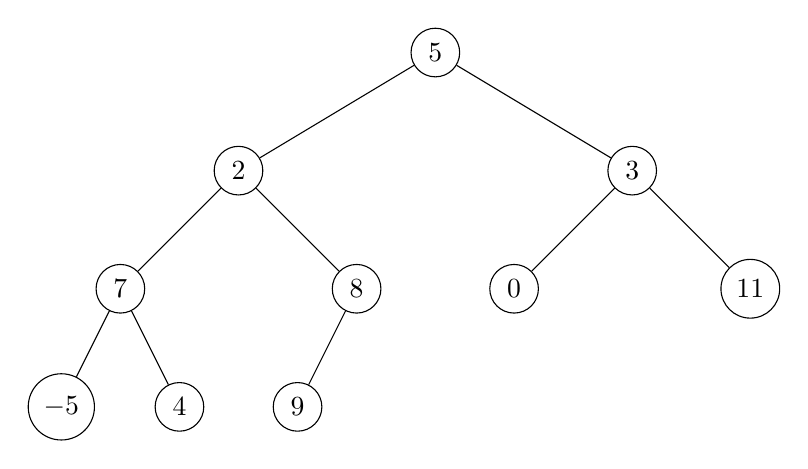
\begin{tikzpicture}[every node/.style={circle,draw},
				level 1/.style={sibling distance=50mm},
				level 2/.style={sibling distance=30mm},
				level 3/.style={sibling distance=15mm}]
\node {5}
child { node {2} 
		child { node {7} 
			child { node {$-5$} }
			child { node {4} }
		} 
		child { node {8} 
			child { node {9} }
			child[missing]
		}
}
child{ node {3}
	child{ node {0} }
	child { node {11} }
};
\end{tikzpicture}
\caption{Oplossing voor de complete binaire boom}
    \label{fig:aug18opl}
\end{figure}
\begin{figure}[htbp]
    \centering
\begin{tikzpicture}[every node/.style={circle,draw},
				level 1/.style={sibling distance=50mm},
				level 2/.style={sibling distance=30mm},
				level 3/.style={sibling distance=15mm}]
\node {5}
child { node {$-3$} 
		child { node {$-4$} 
			child { node {$-8$} }
			child[missing]
		} 
		child { node {3} }
}
child{ node {9}
	child{ node {6} }
	child { node {10} }
};
\end{tikzpicture}
\caption{Deze complete BST bekom je}
    \label{fig:aug18bopl}
\end{figure}
\end{opl}
\end{oef}




\begin{oef}
\papier \emph{(Examen juni 2019)}\\
In onderstaande binaire zoekboom met diepte 5 worden studentendossiers opgeslagen. De dossiers zijn sorteerbaar op familienaam. Er is een dossier voor volgende studenten: Aerts, Bériot, Colins, Decoster, Eerdekens, Lints, Mellaerts, Smolders, Tobback, Vansina. Stel deze namen verkort voor met hun eerste letter: A, B, … , V.

\begin{enumerate}
\item Vul de eerste letter van de 10 namen op de juiste plaats in de BST van figuur~\ref{fig:bstexjuni19}.
\begin{figure}[htbp] 
    \centering
\begin{tikzpicture}[every node/.style={circle,draw},
				level 1/.style={sibling distance=70mm},
				level 2/.style={sibling distance=50mm},
				level 3/.style={sibling distance=30mm},
				level 4/.style={sibling distance=20mm}]
\node {\phantom{T}}
child { node {\phantom{L}} 
	child { node {\phantom{D}} 
		child { node {\phantom{B}}
			child {node {\phantom{A}} }
			child {node {\phantom{C}} }
			} 
		child { node {\phantom{E}} }
		}
	child { node {\phantom{M}} 
		child[missing]  
		child { node {\phantom{S}} }
} }
child { node {\phantom{V}}
	child[missing]
	child[missing]
	};
\end{tikzpicture}
\caption{BST voor studentendossiers}
    \label{fig:bstexjuni19}
\end{figure}


\item Geef \emph{de/een (zie volgende vraag)} volgorde waarin deze 10 dossiers moeten toegevoegd worden. 


\item Is er een andere invoervolgorde mogelijk? Zo ja, geef er één. Zo nee, leg uit waarom er maar één volgorde kan zijn om deze BST te vullen.


\item \emph{(Deze en de volgende vragen kan je pas beantwoorden als de leerstof van heaps gezien is)} Stel dat we deze 10 studentendossiers niet in een BST maar in een binaire max-heap bijhouden. Teken deze binaire max-heap. 

\item Geef de arrayvoorstelling van deze max-heap.

\item Stel dat de binaire max-heap diepte 13 moet hebben. Reken uit hoeveel studentendossiers je dan \emph{minimaal} zou moeten toevoegen bij de boom uit vraag (d). Je mag je berekeningen altijd aan de achterzijde van een blad maken. Verwijs er dan wel duidelijk naar (“zie achterzijde pg …”).
\end{enumerate}
\begin{opl}
Figuur~\ref{fig:bstexjuni19opl} op pagina~\pageref{fig:bstexjuni19opl} toont de BST.
\begin{figure}[htbp] 
    \centering
\begin{tikzpicture}[every node/.style={circle,draw},
				level 1/.style={sibling distance=70mm},
				level 2/.style={sibling distance=50mm},
				level 3/.style={sibling distance=30mm},
				level 4/.style={sibling distance=20mm}]
\node {T}
child { node {L} 
	child { node {D} 
		child { node {B}
			child {node {A} }
			child {node {C} }
			} 
		child { node {E} }
		}
	child { node {M} 
		child[missing]  
		child { node {S} }
} }
child { node {V}
	child[missing]
	child[missing]
	};
\end{tikzpicture}
\caption{BST voor studentendossiers}
    \label{fig:bstexjuni19opl}
\end{figure}
Er zijn vele volgordes mogelijk om deze BST te construeren. Zo kan je laag per laag werken, of er voor kiezen om eerst de linkerboom af te werken en dan de rechter (of omgekeerd). Eén van vele mogelijk volgordes is: T, L, V, D, B, E, A, C, M, S. Het volstaat bvb. om de L en de V van plaats te verwisselen om een andere goede volgorde te bekomen. In arrayvoorstelling geeft dit het volgende (we stellen een lege cel voor door het symbool *): [T, L, V, D, M, *, *, B, E, *, S, *, *, *, *, A, C].

Om deze 10 dossiers voor te stellen in een heap zijn er vele mogelijkheden. Figuur~\ref{fig:bstexjuni19oplheap} op pagina~\pageref{fig:bstexjuni19oplheap} toont er eentje. Om diepte 13 te bereiken moet je veel nodes toevoegen, want de boom moet compleet zijn. Op elk niveau staat een ‘macht van 2’ aantal getallen. Op diepte 4 moeten er $2^3$ knopen zijn. Er staan er al drie, dus je voegt er nog $2^3 - 3$ toe. Op de volgende dieptes voeg je $2^4 + 2^5 + \cdots + 2^{11}$ knopen toe. Tenslotte op diepte 13 nog 1 knoop. We berekenen dus volgende som: 
\[
2^3 - 3 + 2^4 + 2^5 + 2^6 + \cdots + 2^{10} + 2^{11} + 1 = 4086
\]
\begin{figure}[htbp] 
    \centering
\begin{tikzpicture}[every node/.style={circle,draw},
				level 1/.style={sibling distance=70mm},
				level 2/.style={sibling distance=50mm},
				level 3/.style={sibling distance=30mm},
				level 4/.style={sibling distance=20mm}]
\node {V}
child { node {L} 
	child { node {D} 
		child { node {A} } 
		child { node {B} }
	}
	child { node {E} 
		child { node {C} }
		child[missing]
	} 
}
child { node {T}
	child { node {M} }
	child { node {S} }
};
\end{tikzpicture}
\caption{Max-heap voor studentendossiers}
    \label{fig:bstexjuni19oplheap}
\end{figure}
\end{opl}
\end{oef}

\begin{oef}
\papier \emph{(Examen augustus 2017)} Gegeven de boom uit figuur~\ref{fig:boom1ex}.
\begin{figure}[htbp]
    \centering
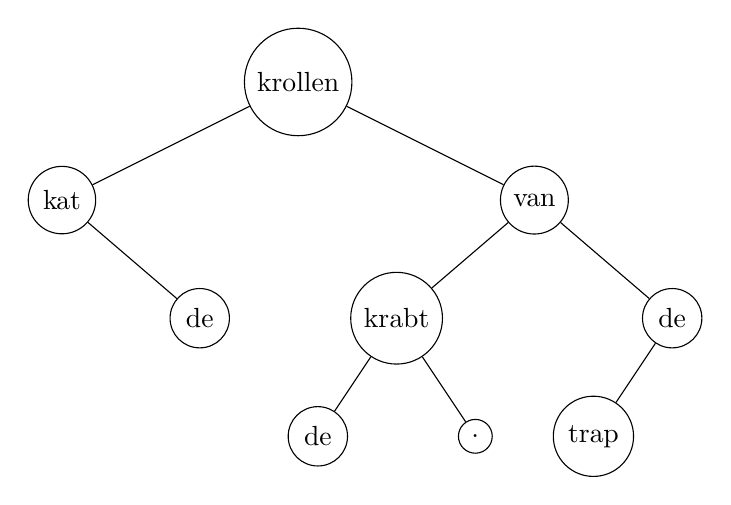
\begin{tikzpicture}[every node/.style={circle,draw},
				level 1/.style={sibling distance=60mm},
				level 2/.style={sibling distance=35mm},
				level 3/.style={sibling distance=20mm}]
\node {krollen}
child { node {kat}
	child [missing] 
	child { node {de}}
	}
child {node {van}
	child{node{krabt}
		child{node{de}}
		child{node{.}}
	}
	child{node{de}
		child{node{trap}}
		child[missing]	
	}
}
;
\end{tikzpicture}
\caption{Boom 1}
 \label{fig:boom1ex}
\end{figure}


\begin{enumerate}
\item Geef de resulterende zin na een inorder-wandeling door de boom van figuur~\ref{fig:boom1ex}. 

\item Gegeven de zin in de vorm van een array van Strings:
\verb+String[]{"Als", "de", "kat",+  \verb+"van", "huis", "is", "dansen", "de", "muizen", "altijd", "op", "tafel"}+. 
\newline
We kunnen deze zin omzetten naar een binaire boom bestaande uit knopen met als dataveld de individuele elementen van deze String-array waarbij een \emph{postorder}-wandeling door deze boom de oorspronkelijke zin teruggeeft. Teken deze boom gegeven dat de boom \emph{compleet} moet zijn.


\end{enumerate}
\begin{opl}
\begin{enumerate}
\item “kat de krollen de krabt . van trap de”
\item Figuur~\ref{fig:dansendemuizen} op pagina~\pageref{fig:dansendemuizen} toont de complete binaire boom.
\begin{figure}[htbp] 
    \centering
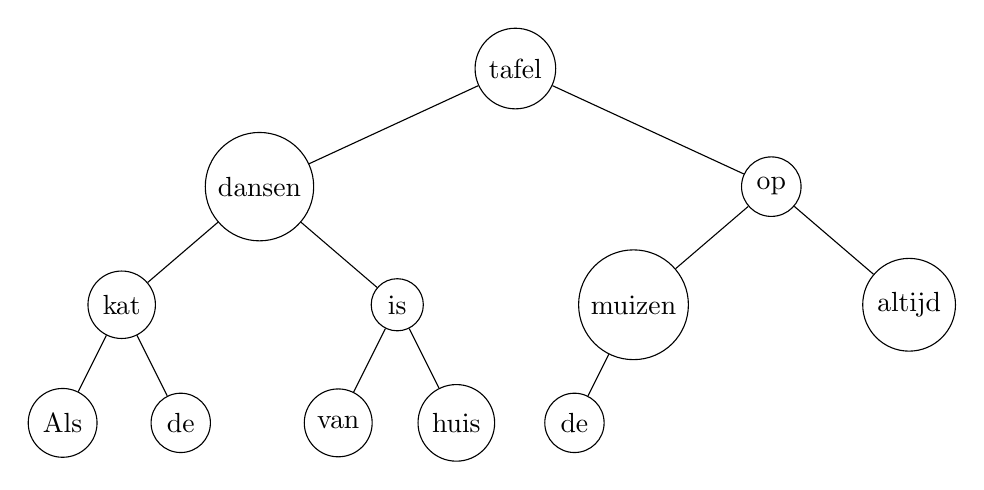
\begin{tikzpicture}[every node/.style={circle,draw},
				level 1/.style={sibling distance=65mm},
				level 2/.style={sibling distance=35mm},
				level 3/.style={sibling distance=15mm},
				level 4/.style={sibling distance=10mm}]
\node {tafel}
child { node {dansen} 
	child { node {kat} 
		child { node {Als} } 
		child { node {de} }
	}
	child { node {is} 
		child { node {van} }
		child { node {huis}	}
	} 
}
child { node {op}
	child { node {muizen} 
		child { node {de} }
		child[missing]
	}
	child { node {altijd} }
};
\end{tikzpicture}
\caption{Als de kat van huis is dansen de muizen altijd op tafel}
    \label{fig:dansendemuizen}
\end{figure}
\end{enumerate}
\end{opl}
\end{oef}





\begin{oef}
\code \emph{(Examen augustus 2017)} Herneem de domainklasse van Binary Tree. Schrijf in deze klasse een methode \verb/deelZonder(E wortelInfo)/ die een nieuwe \verb+BinaryTree<E>+ teruggeeft die gelijk is aan deze boom zonder de deelboom met als wortel de knoop met dataveld wortelInfo. Deze methode geeft \verb+null+ terug indien de parameter niet voorkomt in deze binary tree.

\begin{figure}[htbp]
    \centering
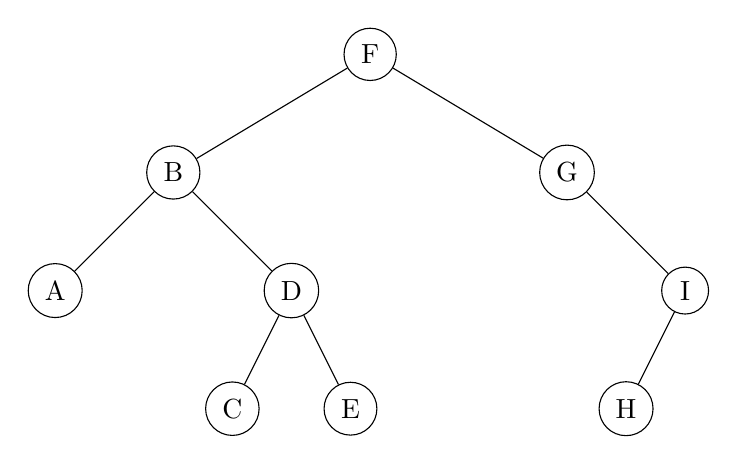
\begin{tikzpicture}[every node/.style={circle,draw},
				level 1/.style={sibling distance=50mm},
				level 2/.style={sibling distance=30mm},
				level 3/.style={sibling distance=15mm}]
\node {F}
child { node {B} 
	child { node {A} }
	child { node {D} 
		child { node {C} } 
		child { node {E} } }
}
child { node {G}
	child[missing]
	child { node {I}
		child { node {H} }
		child[missing] }
};
\end{tikzpicture}
\end{figure}

wordt na het oproepen van de methode \verb+deelZonder(I)+:
\begin{figure}[htbp]
    \centering
\begin{tikzpicture}[every node/.style={circle,draw},
				level 1/.style={sibling distance=50mm},
				level 2/.style={sibling distance=30mm},
				level 3/.style={sibling distance=15mm}]
\node {F}
child { node {B} 
	child { node {A} }
	child { node {D} 
		child { node {C} } 
		child { node {E} } }
}
child { node {G}
};
\end{tikzpicture}
\end{figure}

UI-klasse:
\begin{lstlisting}
public class BinaryTreeDriver {

    public static void main(String[] args) {
        BinaryTree<String> nodeA = new BinaryTree<>("A");
        BinaryTree<String> nodeC = new BinaryTree<>("C");
        BinaryTree<String> nodeE = new BinaryTree<>("E");
        BinaryTree<String> nodeH = new BinaryTree<>("H");
        BinaryTree<String> nodeD = new BinaryTree<>("D", nodeC, nodeE);
        BinaryTree<String> nodeB = new BinaryTree<>("B", nodeA, nodeD);
        BinaryTree<String> nodeI = new BinaryTree<>("I", nodeH, null);
        BinaryTree<String> nodeG = new BinaryTree<>("G", null, nodeI);
        BinaryTree<String> boom = new BinaryTree<>("F", nodeB, nodeG);

        System.out.println("\nVolledige boom preorder:");
        boom.printPreorder();
        System.out.println("\nVolledige boom inorder:");
        boom.printInOrder();

        BinaryTree<String> boomZonderI = boom.deelZonder("I");
        System.out.println("\nBoom zonder I preorder: ");
        boomZonderI.printPreorder();
        System.out.println("\nBoom zonder I inorder: ");
        boomZonderI.printInOrder();

        BinaryTree<String> boomZonderB = boom.deelZonder("B");
        System.out.println("\nBoom zonder B preorder: ");
        boomZonderB.printPreorder();
        System.out.println("\nBoom zonder B inorder: ");
        boomZonderB.printInOrder();
    }

}
\end{lstlisting}

geeft volgende uitvoer:
\begin{lstlisting}
Volledige boom preorder:
F B A D C E G I H 
Volledige boom inorder:
A B C D E F G H I 
Boom zonder I preorder: 
F B A D C E G 
Boom zonder I inorder: 
A B C D E F G 
Boom zonder B preorder: 
F G I H 
Boom zonder B inorder: 
F G H I 
\end{lstlisting}
\begin{opl}
\begin{lstlisting}
   public BinaryTree<E> deelZonder(E wortelInfo) {
        if (wortelInfo == null || !this.contains(wortelInfo))
            return null;
        // wortelInfo == data, dus hele boom verwijderen
        if (this.data == wortelInfo) {
            return null;
        }
        // wortelInfo = linkerkind van data, dus hele linkertak verwijderen
        if (this.leftTree!=null && this.leftTree.data.equals(wortelInfo)){
            return new BinaryTree(this.data,null,this.rightTree);
        }
        // wortelInfo == rechterkind van data, dus hele rechtertak verwijderen
        if (this.rightTree!= null && this.rightTree.equals(wortelInfo)){
            return new BinaryTree(this.data,this.rightTree,null);
        }
        BinaryTree newLeftTree, newRightTree;
        // als wortelInfo in linkertak zit: nieuwe linkertak maken zonder wortelInfo
        if (this.leftTree != null && this.leftTree.contains(wortelInfo))
            newLeftTree = this.leftTree.deelZonder(wortelInfo);
        // anders linkertak behouden
        else newLeftTree = this.leftTree;
        // idem voor rechtertak
        if (this.rightTree!=null && this.rightTree.contains(wortelInfo))
            newRightTree = this.rightTree.deelZonder(wortelInfo);
        else
            newRightTree = this.rightTree;
        // resulterende boom terug samenstellen
        return new BinaryTree<>(this.data,newLeftTree,newRightTree);
    }
\end{lstlisting}
\end{opl}
\end{oef}




\begin{oef}
\code \emph{(Examen juni 2018)} We noemen een binaire boom \emph{strikt} als alle knopen ofwel 0 ofwel 2 (dus niet 1!) kinderen hebben. Schrijf een methode \verb+isStrikt(): boolean+ die van een gegeven binaire boom nakijkt of hij strikt is. 

Vertrek van de klasse \verb+BinaryTree<E>+ die we definieerden in de les:
\begin{lstlisting}	
package domain;

import java.util.ArrayList;

public class BinaryTree<E> {
	private E data;
	private BinaryTree<E> leftTree, rightTree;
	
	public BinaryTree(E data){
		this(data,null,null);
	}
	
	public BinaryTree(E data, BinaryTree<E> leftTree, BinaryTree<E> rightTree){
		this.data= data;
		this.leftTree= leftTree;
		this.rightTree= rightTree;
	}
}
\end{lstlisting}

Maak in het package \verb+ui+ een \verb+main+ methode in het bestand \verb+BinaryTreeDriver.java+ om de boom uit figuur~\ref{fig:boom1exjuni19} te maken.
\begin{figure}[htbp]
    \centering
\begin{tikzpicture}[every node/.style={circle,draw},
				level 1/.style={sibling distance=50mm},
				level 2/.style={sibling distance=30mm},
				level 3/.style={sibling distance=20mm}
]
\node {J}
child { node {$E$} 
	child { node {R} } 
	child { node {P} } }
child { node {$A$} 
	child { node {G} } 
	child { node {F} 
		child{node{M}}
		child [missing]{}
		}
	};
\end{tikzpicture}
\caption{Eenvoudige binaire boom van gehele getallen}
    \label{fig:boom1exjuni19}
\end{figure}

Zorg dat je \verb+main+ methode volgend resultaat in de console toont:
\begin{verbatim}
volledige binaire boom strikt? -> false
binaire boom met enkel node R strikt? -> true
binaire boom met node E en kinderen R en P strikt? -> true
\end{verbatim}
\begin{opl}
\begin{lstlisting}
   public boolean isStrict() {
        // wortel == blaadje
        if (this.isLeaf())
            return true;
        // wortel heeft linker- en rechtertak, dus rest van boom controleren
        if ((this.leftTree != null && this.rightTree != null)) {
            return this.leftTree.isStrict() && this.rightTree.isStrict();
        }
        // bij wortel ontbreekt linker- of rechtertak
        return false;

    }
    \end{lstlisting}
\end{opl}
\end{oef}



\begin{oef}
\code \emph{(Examen juni 2019)} Gegeven een BST zoals we die implementeerden in de les. Schrijf een methode \verb+geefKnopenBinnenInterval(min:E, max:E): ArrayList<E>+ die een arraylist geeft van alle knopen in stijgende volgorde en gelegen binnen het interval \verb+[min,max]+. 

UI klasse:
\begin{lstlisting}
    public static void main(String[] args) {
        BinarySearchTree<Integer> boom = new BinarySearchTree<>();
        boom.addNode(6);
        boom.addNode(4);
        boom.addNode(8);
        boom.addNode(3);
        boom.addNode(5);
        boom.addNode(7);
        boom.addNode(9);

        printBoomInfo(boom);

        System.out.println("\nKnopen tussen 5 en 8: "+boom.geefKnopenBinnenInterval(5,8));
        System.out.println("\nKnopen tussen 3 en 5: "+boom.geefKnopenBinnenInterval(3,5));
        System.out.println("\nKnopen tussen 8 en 9: "+boom.geefKnopenBinnenInterval(8,9));
        System.out.println("\nKnopen tussen -10 en 0: "+boom.geefKnopenBinnenInterval(-10,0));
        System.out.println("\nKnopen tussen 100 en 110: "+boom.geefKnopenBinnenInterval(100,110));
\end{lstlisting}
geeft volgende uitvoer:
\begin{lstlisting}
Knopen tussen 5 en 8: [5, 6, 7, 8]

Knopen tussen 3 en 5: [3, 4, 5]

Knopen tussen 8 en 9: [8, 9]

Knopen tussen -10 en 0: []

Knopen tussen 100 en 110: []
\end{lstlisting}
\begin{opl}
Werkwijze: Bekijk de code van de methode \verb/printInOrder()/. In die methode schrijf je eerst recursief de waarden uit van de linkerboom, dan de waarde van de wortel, dan behandel je de rechterboom. Hier kan je ook zo te werk gaan. De waarden zullen dan van klein naar groot geordend zijn. 

In tegenstelling tot \verb/printInOrder()/ schrijven we de waarden nu niet uit naar de console, maar verzamelen we ze in een lijst. Dat is gelijkend op hetgeen je deed in de methode \verb/getDataLeaves()/. 

Tenslotte hoef je niet steeds te zoeken over het volledige interval. Immers, in een BST zijn de elementen links van wortel kleiner dan wortel en rechts ervan groter. Je kan het interval waarin je zoekt dus steeds kleiner maken.

\begin{lstlisting}
public class BinarySearchTree<E extends Comparable<E>> {
    private BinaryTree<E> root;

   ...
   
       public List<E> geefKnopenBinnenInterval(E min, E max) {
        if (this.isEmpty())
            throw new IllegalStateException("Empty tree");
        return this.root.geefKnopenBinnenInterval(min, max);
    }

    private class BinaryTree<E extends Comparable<E>> {
        private E data;
        private BinaryTree<E> leftTree, rightTree;

	...
	
	        public List<E> geefKnopenBinnenInterval(E min, E max) {
            if (min == null || max == null)
                throw new IllegalArgumentException("Geen effectief interval");
            List<E> result = new ArrayList<>();
            if (min.compareTo(max) > 0)
                return result;
                
                // zoek eerst waarden in linkerboom
                // je hoeft niet over volledig interval te zoeken 
                // want alle knopen in linkerboom zijn kleiner dan wortel
            if (this.leftTree != null)
                result.addAll(this.leftTree.geefKnopenBinnenInterval(min, getMinimum(this.data, max)));
                // controleer of data in gevraagde interval zit
            if (this.data.compareTo(min) >= 0 && this.data.compareTo(max) <= 0)
                result.add(this.data);
                // behandel rechterboom
            if (this.rightTree != null)
                result.addAll(this.rightTree.geefKnopenBinnenInterval(getMaximum(min, this.data), max));
            return result;
        }

        private E getMinimum(E object1, E object2) {
            if (object1.compareTo(object2) <= 0)
                return object1;
            else
                return object2;
        }

        private E getMaximum(E object1, E object2) {
            if (object1.compareTo(object2) >= 0)
                return object1;
            else
                return object2;
        }
    }
\end{lstlisting}
\end{opl}
\end{oef}


